\documentclass[10pt]{report}
\usepackage[a4paper, height=10in, width=8in, hmargin={2cm,0.8in}]{geometry}
\usepackage{graphicx} % Required for inserting images
\usepackage{xeCJK}
\usepackage{amssymb}
\usepackage{amsthm}
\usepackage{amsmath}
\usepackage{caption}
\usepackage{comment}
\usepackage{subcaption}
\usepackage{enumerate}
\usepackage{multirow}
\usepackage{physics}
\usepackage[separate-uncertainty=true]{siunitx}
\usepackage{multirow}
\usepackage{booktabs}
\usepackage{chemformula}
\usepackage{sectsty}
\usepackage{svg}
\usepackage{url}
\usepackage{titlesec}
\usepackage{fontenc}

\newcommand{\chapfnt}{\fontsize{16}{19}}
\titleformat{\chapter}[hang]
{\normalfont\chapfnt\bfseries}{\thechapter}{20pt}{\chapfnt}

\setCJKmainfont{NotoSansTC-Regular}
\renewcommand{\baselinestretch}{1.25}

\title{112-2 近代物理實驗\\Ultrasonic Comprehensive\\\vspace{1cm}
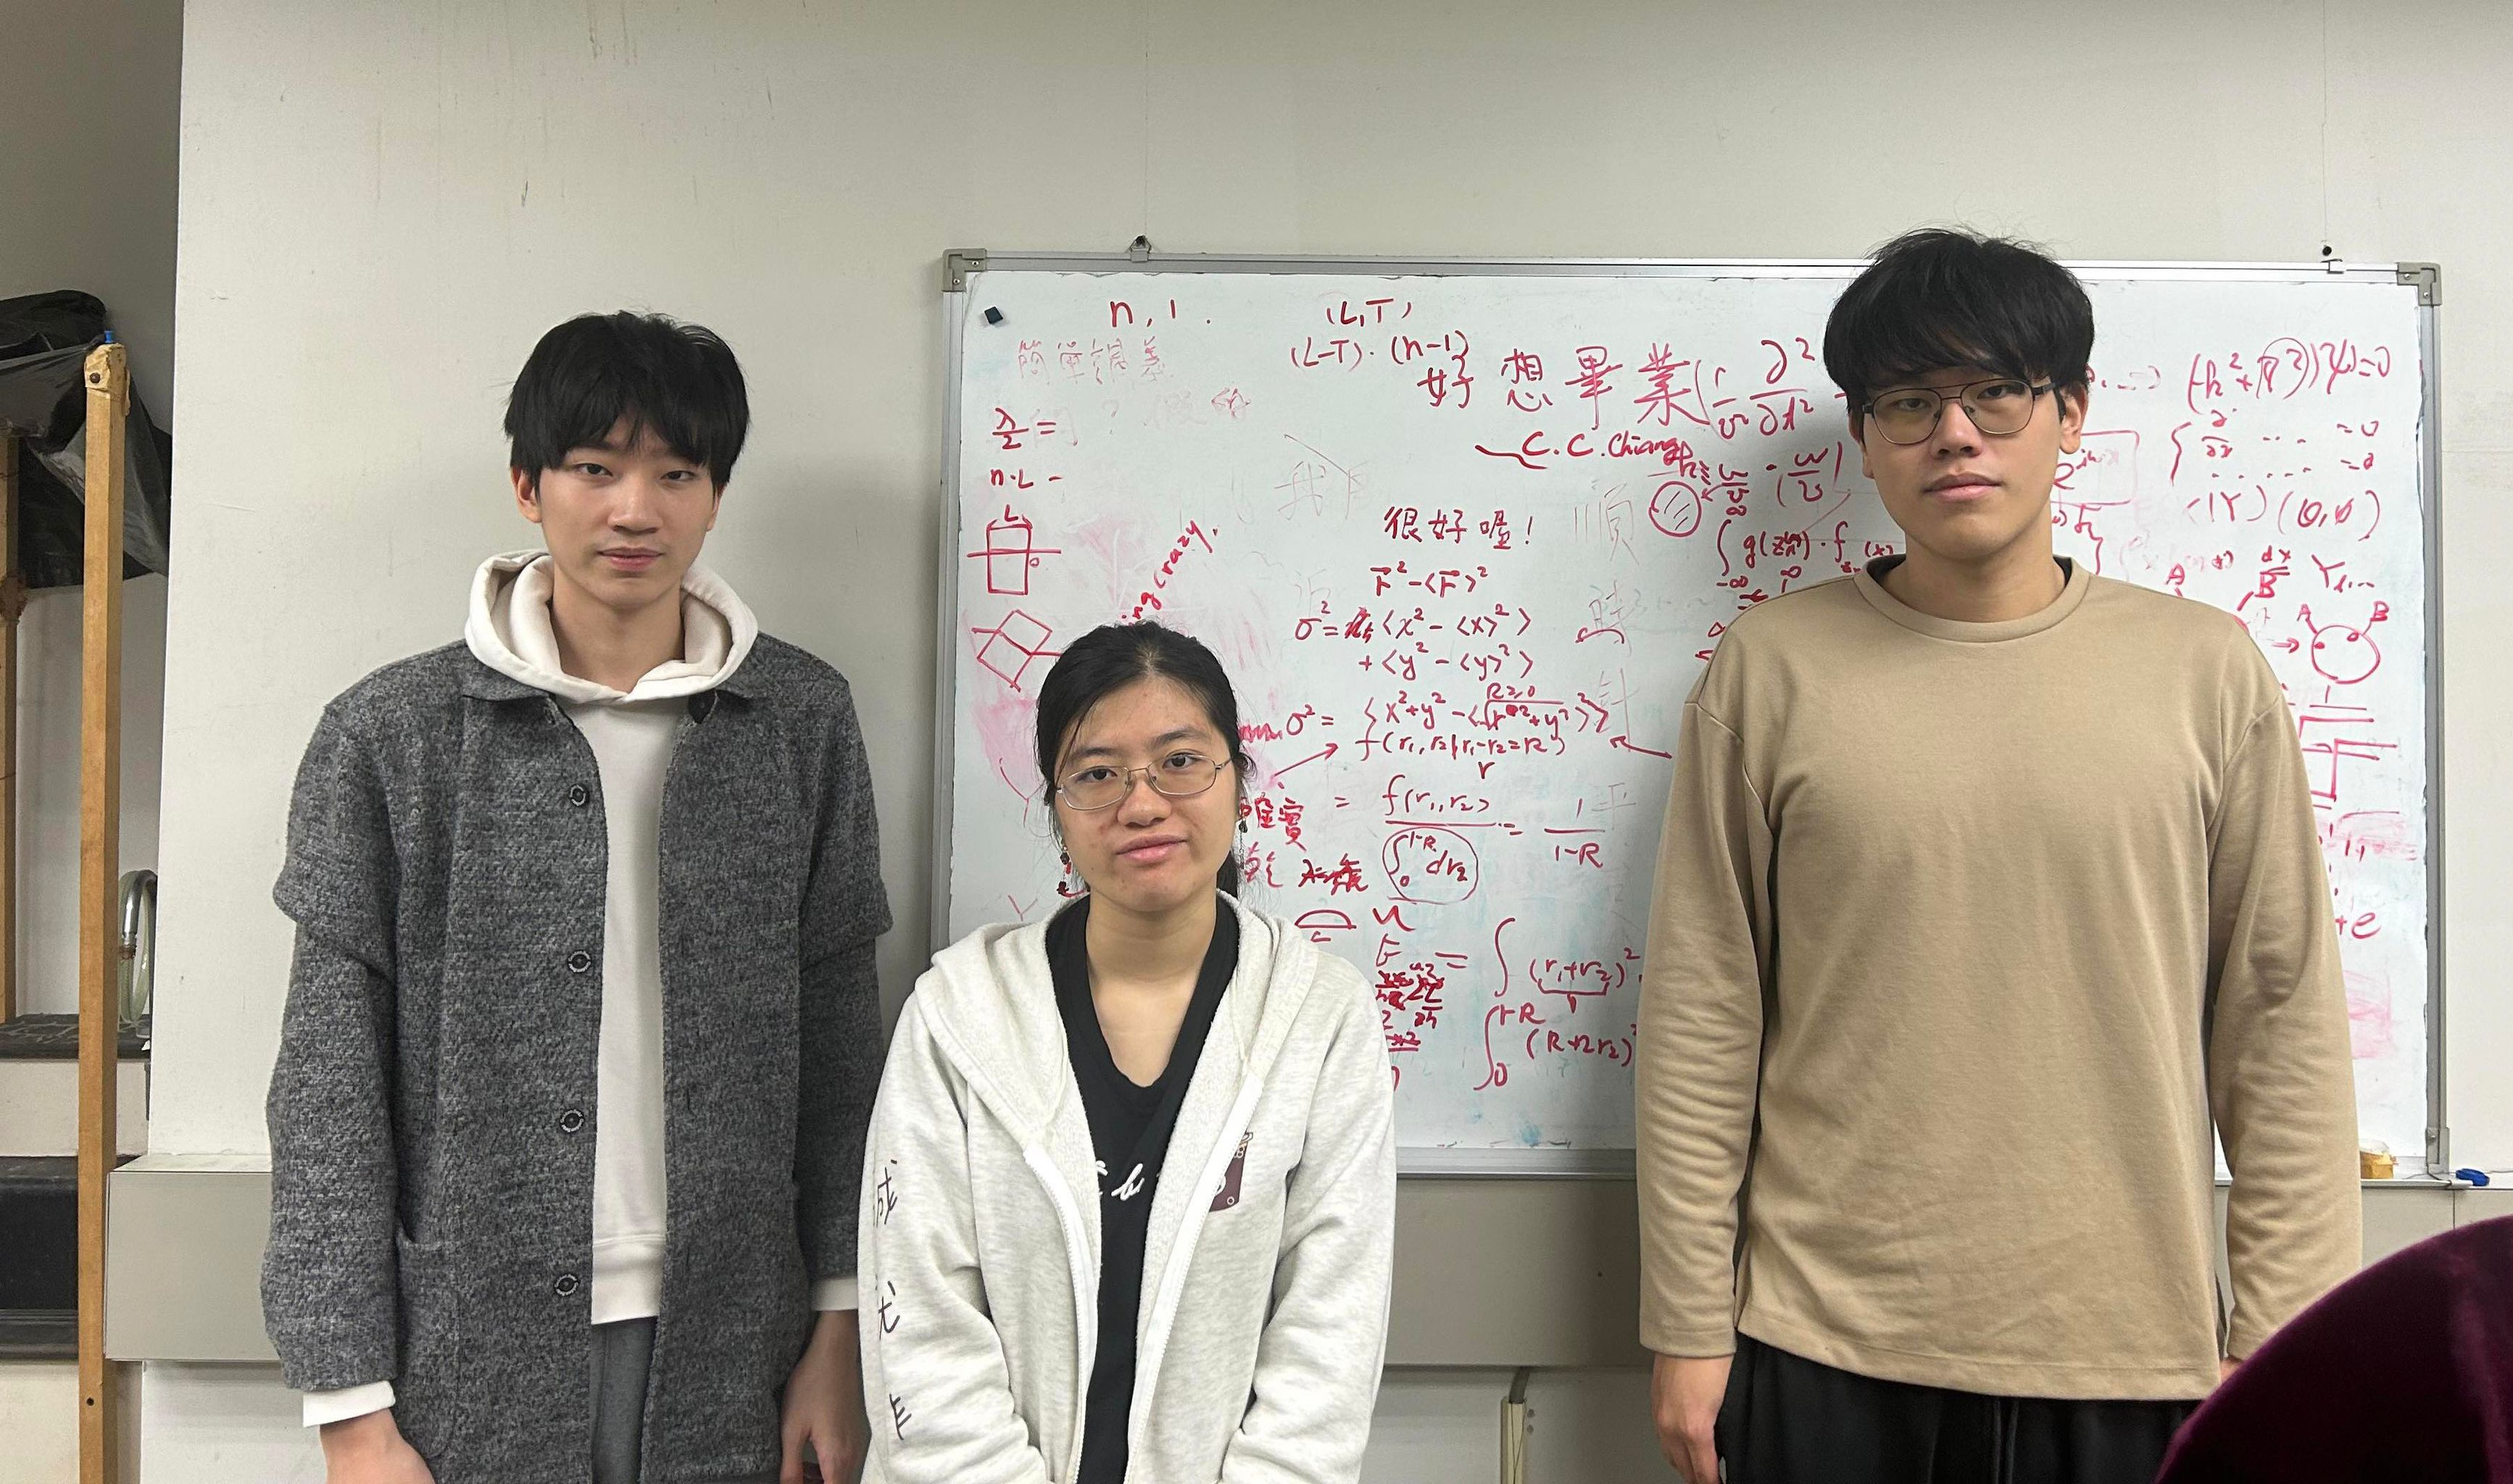
\includegraphics[width=0.5\textwidth]{Group photo}
}
\author{週一班第二組 \\ 左:林馳耘 B10202037 中:吉芸萱 B10202036 右:丁安磊 B10202051}
\date{實驗日期:04/29, 05/06, 05/07/2024\\提交日期: 05/20/2024}

\begin{document}

\renewcommand{\figurename}{圖}
\renewcommand{\tablename}{表}
\newcommand{\br}[1]{\left(#1\right)}
\renewcommand{\vb}[1]{\boldsymbol{\mathbf{#1}}} % New vector bold command to adapt for greek letters.

\maketitle

\tableofcontents

\clearpage

\section{引言與原理}

\chapter{PHY04 Attenuation of ultrasound in liquids}

\chapter{PHY23 Dispersion of ultrasonic waves (Lamb waves)}

\section{引言與原理}

\subsection{Lamb Wave}

將質點的位移$\vb{u}=(u,v,w)$ 透過Helmholtz 分解寫成
\begin{equation}
    \vb u=\nabla\phi+\nabla\times\vb\psi;\quad \nabla\vb\psi=0
\end{equation}
代入彈性材料中的運動方程
\begin{equation}
    \mu \nabla^2 \vb{u} + (\lambda+\mu)\nabla\nabla\cdot \vb{u}=\rho \ddot{\vb{u}}
\end{equation}
可以得到
\begin{equation}
    \nabla\left[(\lambda+2\mu)\nabla^2\phi-\rho\ddot{\phi}\right]
    +\nabla\times\left[\mu\nabla^2\vb\psi-\rho\vb{\ddot{\vb{\psi}}}\right]=0
\end{equation}
\begin{align}
    \nabla^2\phi-\frac{1}{c_L^2}\ddot{\phi}&=0,\quad c_L^2=\frac{\lambda+2\mu}{\rho} \\
    \nabla^2\vb{\psi}-\frac{1}{c_T^2}\ddot{\vb{\psi}}&=0,\quad c_T^2=\frac{\mu}{\rho}
\end{align}
$\phi=\phi(x,z), \vb\psi=(0,-\psi_y(x,z),0)$
考慮以下形式的解
\begin{align}
    \phi&=\Lambda(z)e^{i(kx-\omega t)} \\
    \psi_y&=\Omega(z)e^{i(kx-\omega t)}
\end{align}
\begin{align}
    \text{S mode: } & \Lambda(z)=A\cos(\alpha z),\quad \Theta(z)=B\sin(\beta z) \\
    \text{A mode: } & \Lambda(z)=A\sin(\alpha z),\quad \Theta(z)=B\cos(\beta z) \\
\end{align}

\begin{align}
    \alpha^2&=\left(\frac{\omega}{c_L}\right)^2-k^2 \\
    \beta^2&=\left(\frac{\omega}{c_T}\right)^2-k^2 
\end{align}
\begin{equation}
    \frac{\tan(\beta h)}{\tan(\alpha h)}=\left[ 
    \frac{4k^2\alpha\beta}{(k^2-\beta^2)^2}
    \right]^{\pm 1}
\end{equation}
+1: S, -1: A
\section{實驗步驟}

本實驗使用 1 MHz、2 MHz、4 MHz 的 probe,調整至 transmission 
mode。藉由兩個 probe 搭配不同角度及底座厚度的薄板,來觀察不同模
態的 lamb waves。首先用游標尺測量薄板厚度,並在使用不同 probe 時
讀取測量當下的實際頻率。

 測量群速度時,先以兩 probe 靠最近時的位置為基準點,紀錄此時
的傳播時間 $t_0$,接著拉開兩 probe 距離 $x_1$,訊號抵達的時間會往後退,
此時紀錄新的傳播時間 $t_1$,而超聲波在薄板中傳播的群速度則為 $v_{\rm g}= 
x_1/(t_1-t_0)$。
 本實驗需測量的 lamb wave 模態與對應的 probe 頻率如下:
\begin{table}[ht]
\centering
\caption{本實驗使用的激發頻率與入射角組合與對應的主要受激模態}
\label{tab:my-table}
\begin{tabular}{@{}cccll@{}}
\toprule
\multicolumn{1}{l}{玻璃厚度$d$} & \multicolumn{1}{l}{}    & 入射角$\alpha_{\rm W}$                  & 激發頻率 & 模態 \\ \midrule
\multirow{8}{*}{1 mm}    & \multirow{2}{*}{LW1}    & \multirow{2}{*}{12°} & 2 MHz         & A1     \\
                         &                         &                      & 4 MHz         & S2     \\ \cmidrule(l){2-5} 
                         & \multicolumn{1}{l}{LW2} & 15°                  & 2 MHz         & A1     \\ \cmidrule(l){2-5} 
                         & \multirow{2}{*}{LW3}    & \multirow{2}{*}{28°} & 2 MHz         & S0     \\
                         &                         &                      & 4 MHz         & A1     \\ \cmidrule(l){2-5} 
                         & \multicolumn{1}{l}{LW4} & 32°                  & 4 MHz         & A1     \\ \cmidrule(l){2-5} 
                         & \multirow{2}{*}{LW5}    & \multirow{2}{*}{35°} & 1 MHz         & S0     \\
                         &                         &                      & 2 MHz         & S0     \\ \midrule
\multirow{3}{*}{1.3 mm}  & \multirow{2}{*}{LW6}    & \multirow{2}{*}{25°} & 1 MHz         & S0     \\
                         &                         &                      & 2 MHz         & A1     \\ \cmidrule(l){2-5} 
                         & \multicolumn{1}{l}{LW7} & 32°                  & 2 MHz         & S0     \\ \bottomrule
\end{tabular}
\end{table}

\subsubsection{觀察}

\section{結果與討論}

游標尺最小單位\SI{0.02}{mm},因此B類不確定度為$\SI{0.02}{mm}/\sqrt{3}=\SI{0.01}{mm}$

PHY06: \SI{80.46(1)}{mm},\SI{150.44(1)}{mm},\SI{42.00(1)}{mm}










\section{回答問題}

\newcommand\question[1]{
  \fbox{\parbox{\dimexpr\linewidth - 2\fboxrule - 2\fboxsep}{#1}}\vspace{2mm}
}

\subsection{問題一}\label{Q1}

\question{
}

\chapter{結論}

\appendix

\chapter{附錄}

\section{附錄:參考的理論值}

\section{附錄:數據分析的程式部分}

本次實驗報告使用的 Python 進行數據的讀取與分析,列舉幾個其中主要的 package 與函式如下:
\begin{itemize}
    \item \verb|scipy.optimize.curve_fit|: 用於擬合包絡線方程式,指定模型$y=f(x,\vb{\alpha})$後給定$(x,y)$數據點回傳最佳的參數$\vb{\alpha}$的值與共變異數矩陣(其對角元素能用來估計參數的不確定度。)
    \item \verb|scipy.fft.fft, fftfreq, ifft|: 進行快速傅立葉變換與其逆變換。
    \item \verb|sklearn.metrics.r2_score|: 計算線性回歸模型的$R^2$值
    \item \verb|uncertainties.ufloat|: 包含最佳估計值與不確定的浮點數值,對其直接進行運算可以得到不確定度傳遞的結果。
\end{itemize}

\bibliographystyle{unsrt} % We choose the "plain" reference style
\bibliography{ref.bib} % Entries are in the refs.bib file

\end{document}